\section{Case Study}
%\label{sec:case_study}

In this section, we describe the datasets used in this experiment and the experiment environment.
Also, we report the results of our forecasting model.
In our experiments, our model was able to efficiently forecast the flow of human crowds by using three datasets: (1)~Trajectory data extracted from Twitter, (2)~Human trajectory data (GeoLife) ~\cite{Zheng:2009:Mining}, and (3)~Taxi location data~\cite{NYC:2016:Taxi}.
Details on these three datasets have been provided in this section. 
%We now provide details on these ... WHAT?

\subsection{Twitter Data}
%A growing number of people use using 
Location-based social network services (e.g., Twitter, Instagram) have become ubiquitous in the modern age.
They create geo-located data and share this information about their immediate surroundings using smart phones with GPS.
Such spatiotemporal data is also a great data source to understand human mobility.
In this work, we use geo-located twitter data.
We mainly focus on the data generated within Manhattan.
Figure~\ref{fig:twitter_flow} shows an example of the flow results from Twitter data generated in the morning between 6:00 AM - 10:00 AM of August 30th, 2014.
We can see major flows toward from top-right to bottom-left and gathering at the center of Manhattan (See Figure~\ref{fig:twitter_flow} (A)).
Figure~\ref{fig:twitter_flow} (B) shows the probability flow of the same region.
We can see high uncertainty around the center as complex movements.
Figure~\ref{fig:twitter_flow_prediction} shows the forecast result of the same time window as the result of Figure~\ref{fig:twitter_flow}.
The forecast results of the two visualization show significantly similar patterns to the actual result patterns.



\subsection{GeoLife Data: GPS Trajectory Data}

The GeoLife GPS Trajectory Dataset~\cite{Zheng:2009:Mining} contains a total of 18,670 trajectories from 182 users recorded by Microsoft Research Asia (MSRA) in the Beijing from April 2007 to August 2012.
As the data has a high degree of sparseness, we use a longer time window unit (8 hours) and a longer range of historical data (150 days) than with the other example datasets.
Also, when the grid size is less than 500 meters, we cannot compute the future flows, because the size created too many sub-spaces with no data (trajectory).
Figure~\ref{fig:geolife_example} shows an example of the flow results from GeoLife data generated during the evening between 4:00 PM - 10:00 PM on April 22nd, 2009.
The MSRA is located in the center of the highlighted region in Figure~\ref{fig:geolife_example}.
Figure~\ref{fig:geolife_example}~(A) shows the traffic leaving the MSRA campus, because the observed time window is the evening.
The flows of Figure~\ref{fig:geolife_example}~(B) shows the forecast result of the same time window.
We can see also similar pattens in the both actual and forecast flows.
We zoom into the region highlighted in Figure~\ref{fig:geolife_example} and show the probability flow of the zoomed region in Figure~\ref{fig:geolife_msra}.
The flow appears to show masive complex movements around this area.

\begin{figure*}[tb]
	\centering
	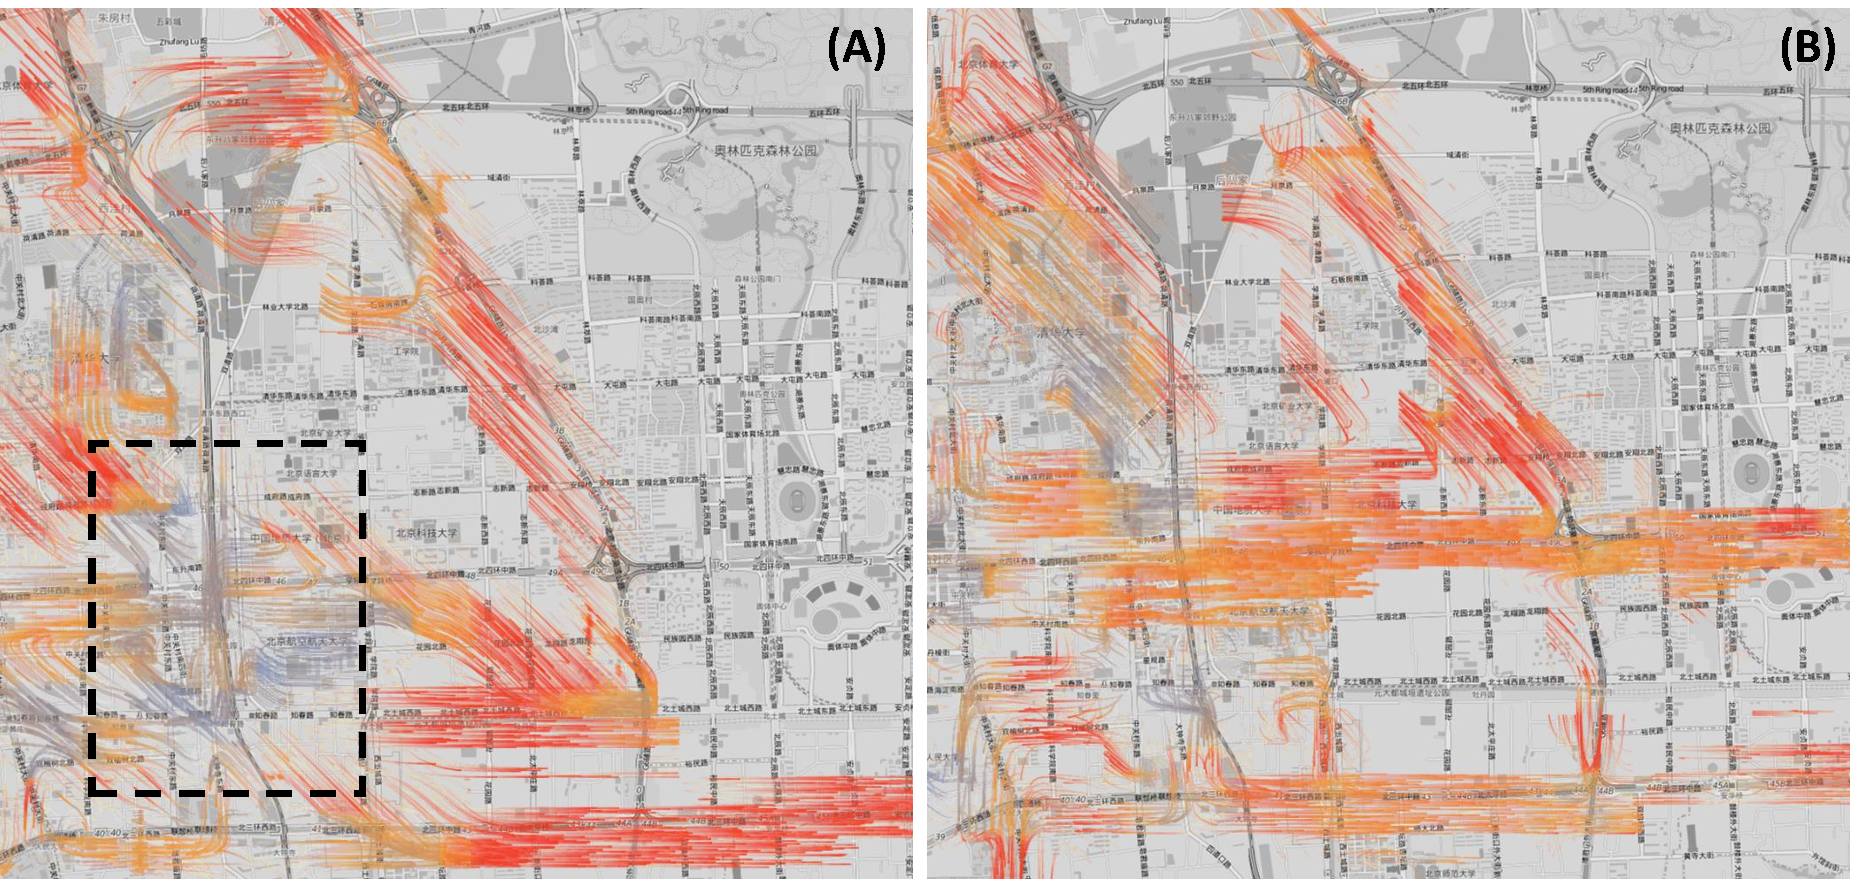
\includegraphics[width=1.0\linewidth]{geolife_example}
	\caption{Flow around the MSRA campus located in the center of the highlighted region. It shows the major flow from GeoLife data during the evening between 4:00 PM - 10:00 PM on April 22nd, 2009. Actual Flow (A) and Forecast Flow (B)}
	\label{fig:geolife_example}
	%\vspace{-0.7cm}
\end{figure*}


\begin{figure}[tb]
	\centering
	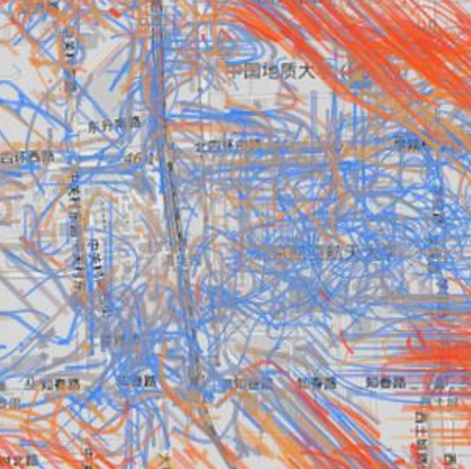
\includegraphics[width=0.6\columnwidth]{geolife_msra}
	\caption{The probability flow zoomed in the MSRA campus}
	\label{fig:geolife_msra}
\end{figure}


\subsection{New York Taxi Data}

The taxi data collected by the New York City (NYC) Taxi and Limousine Commission contains historical taxi trips in NYC, with an average of 500,000~trips per day~\cite{NYC:2016:Taxi}.
Each trip includes passenger pickup and drop-off locations and times, along with other meta data (e.g., trip distance, fare amount).
To demonstrate our work, we utilize the location and time information from the taxi data and focus mainly on trips that took place in Manhattan in 2013.
%For Twitter and taxi data, we looked at the same geo-boundary.
%The taxi data has a more frequent sampling rate than the Twitter data, and the 
%has less uncertainty than twitter data, we used the taxi data for verify results from twitter data.
%We can see the results from both datasets are very similar patterns [FIGURE].
We utilize 1 year of historical data (aggregated by day), and filter the data for portions of the day (i.e., by hour-of-the-day) and utilize our forecasting methodology described in Section~\ref{sec:futureflow}.
We generate these forecasts for three time ranges for 5/30/2013 (Monday): (1) Morning rush hour (6~am~-~9am) (Figure~\ref{fig:case_study_taxi}~(Left)), (2) Afternoon (lunch) commute (11~am~-~2pm) (Figure~\ref{fig:case_study_taxi}~(Middle)), and (3) Evening rush hour (4~pm~-~7pm) (Figure~\ref{fig:case_study_taxi}~(Right)).

The morning commute results (Figure~\ref{fig:case_study_taxi}~(Left)) show an overall pattern of people moving into the middle and southern regions of Manhattan.
This conforms with what is expected and shows that people commute to the commercial regions of the city.
The evening commute results (Figure~\ref{fig:case_study_taxi}~(Right)) show the opposite patterns, and indicate that people may be traveling from work back to home.
The patterns observed during the lunch hours represents more uncertainty of the flows as shown the highlighted region in Figure~\ref{fig:case_study_taxi}~(Middle).
However, we notice more local trends in these results.
%DISCUSS MORE LOCAL TRENDS HERE.
Figure~\ref{fig:case_study_taxi_sub} shows the probability flow of the area highlighted in Figure~\ref{fig:case_study_taxi}~(Left) within the same time frames.
We also note that the forecasts indicate less taxi traffic utilizing the Lincoln tunnel highlighted in Figure~\ref{fig:case_study_taxi_sub}~(Middle) during the morning and evening rush hours. 
However, the Lincoln tunnel is found to have a higher predicted flow during lunch commute hours (Figure~\ref{fig:case_study_taxi_sub}~(Middle)); thereby, indicating that taxi drivers prefer to avoid the tunnel during the morning and evening rush hours.

\begin{figure*}[tb]
	\centering
	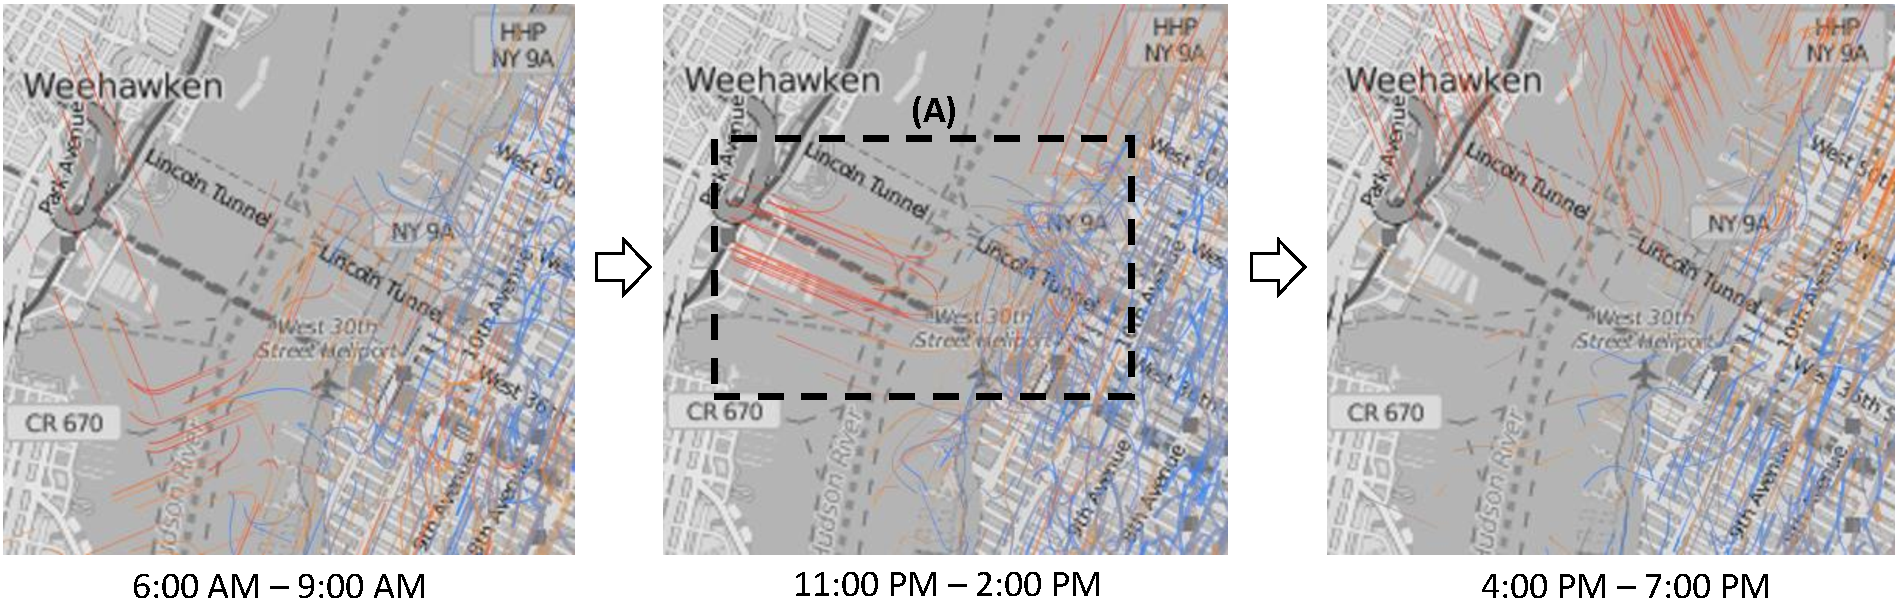
\includegraphics[width=1.0\linewidth]{case_study_sub}
	\caption{The probability flow zoom in around the Lincoln tunnel. Less taxi traffic utilizing the tunnel during the morning (left) and evening (right) rush hours. However, there is a higher predicted flow during lunch commute hours (middle).}
	\label{fig:case_study_taxi_sub}
\end{figure*}


\subsection{Effect of Parameters}

Our trajectory data modeling process for Twitter data introduces several limitations, including issues that arise due to data sparsity. 
In order to mitigate for these challenges, we utilize our flow smoothing approach as described in Section~\ref{sec:smoothing}.
Figure~\ref{fig:LessSmoothing} provide results of applying different global $\tau$ and local $\lambda$ smoothing operations.
The flow with low parameters shows less smooth flow in Figure~\ref{fig:LessSmoothing}~(A) than the flow with high parameter values in in Figure~\ref{fig:LessSmoothing}~(B).

\begin{figure}[tbh]
	\centering
	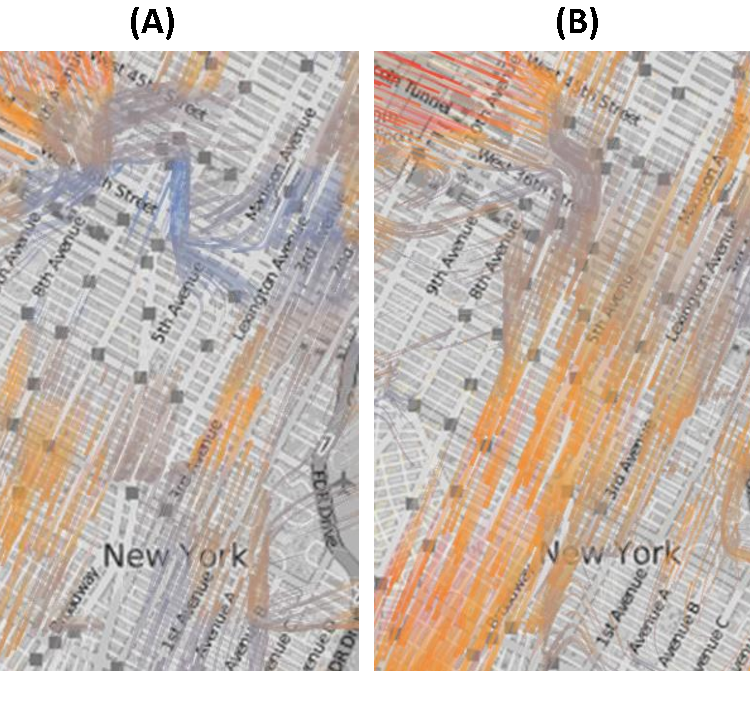
\includegraphics[width=1.0\columnwidth]{LessSmoothing}
	\caption{Smoothing Effect: The flow with the low local smoothing parameter ($\lambda = 0.1$ and $\tau = 0.1$) (A). The flow with the high local smoothing parameter ($\lambda = 0.5$ and $\tau = 0.5$) (B)}
	\label{fig:LessSmoothing}
\end{figure}